% !TeX spellcheck = de_DE_frami
%%%%%%%%%%%%%%%%%%%%%%%%%%%%%%%%%%%%%%%%%%%%%%%%
% COPYRIGHT: (C) 2012-2015 FAU FabLab and others
% Bearbeitungen ab 2015-02-20 fallen unter CC-BY-SA 3.0
%%%%%%%%%%%%%%%%%%%%%%%%%%%%%%%%%%%%%%%%%%%%%%%%

\newcommand{\basedir}{fablab-document}
\documentclass{\basedir/fablab-document}

\usepackage{caption}
\usepackage{textcomp} % \textcelsius
\usepackage{tabularx} % Tabellen mit bestimmtem Breitenverhältnis der Spalten
\usepackage{float} % Ermöglicht H als Platzierungsoption
\usepackage{qrcode}
\usepackage{betriebsanweisung/ba-layout}

% Stammdaten der Betriebsanweisungen
% (Inhalt: betriebsanweisung/inhalt_gktwo.tex und betriebsanweisung/inhalt_resin.tex)
% =====================================================================
%  Stammdaten der Betriebsanweisungen
%  (eingebunden von SLA_Drucker_Einweisung.tex)
%  Gerät, Gerätebilder und BA-Nummer stehen in inhalt_gktwo.tex bzw.
%  inhalt_resin.tex.
% =====================================================================
\renewcommand{\BAfirma}{FAU FabLab, Friedrich-Alexander-Universität Erlangen-Nürnberg}
\renewcommand{\BAlogo}{FabLab_Logo}
\renewcommand{\BAbereich}{Raum U1.239, Hörsaalgebäude (MHB), Erwin-Rommel-Str.\ 60, 91058 Erlangen}
\renewcommand{\BAdatum}{28.09.2026}
\renewcommand{\BAverantw}{Name der verantwortlichen Person}


\newcommand{\ra}{$\Rightarrow$}

\date{\today}
% Versionsnummer: version.tex wird von der GitHub Action erzeugt,
% lokal steht stattdessen "Entwurf" mit Datum in der Fußzeile.
\InputIfFileExists{version}{}{\newcommand{\Version}{Entwurf \today}}
\fancyfoot[R]{Version \Version}
\author{kontakt@fablab.fau.de}
\title{Einweisung SLA 3D-Drucker}

\begin{document}

\maketitle
\begin{center}
	Für den Resin-3D-Drucker \textbf{UniFormation GKtwo}\\
	mit \textbf{Lychee Slicer} und \textbf{Phrozen Water-Washable Rapid Black}\\[1mm]
	{\small Version \Version}
\end{center}

\textbf{Nur eingewiesene Benutzer dürfen den Drucker selbstständig benutzen.}
Wenn du noch nicht eingewiesen bist, frage einen Betreuer. Nach der Einweisung und Unterschrift darfst du den Drucker selbstständig verwenden.

\section{Regeln und Sicherheit}

\begin{itemize}
	\item Die grüne \textbf{UV-Schutzhaube} bleibt während des Drucks geschlossen. Schau ab und zu durch die Haube, ob der Druck gut läuft.
	\item Drucke dürfen auch \textbf{über Nacht} laufen. Wenn du vor dem Druckende gehst, klebe einen \textbf{Post-it mit deinem Namen und deiner E-Mail-Adresse} an den Drucker.
	\item Greife nicht in den Tank, solange sich die Plattform bewegt. Spitze Gegenstände haben im Tank nichts zu suchen, denn die \textbf{nFEP-Folie} und das LCD darunter sind empfindlich.
	\item Es wird nur \textbf{Phrozen Water-Washable Rapid Black} verwendet. Harz füllst du nur nach Absprache mit einem Betreuer nach, die Wartung übernehmen die Betreuer.
	\item \textbf{Vergiss das Bezahlen nicht.}
\end{itemize}

\subsection{Gefahren und Schutzausrüstung}

\begin{center}
	\includegraphics[height=11mm]{GHS05}\quad
	\includegraphics[height=11mm]{GHS07}\quad
	\includegraphics[height=11mm]{GHS08}\quad
	\includegraphics[height=11mm]{GHS09}\qquad\qquad
	\includegraphics[height=11mm]{M004}\quad
	\includegraphics[height=11mm]{M009}
\end{center}

\begin{itemize}
	\item Das flüssige Harz verursacht \textbf{schwere Augenschäden}, reizt die Haut und \textbf{kann Allergien auslösen}, die ein Leben lang bleiben.
	\item Das Harz \textbf{kann die Fruchtbarkeit beeinträchtigen und das Kind im Mutterleib schädigen}. \textbf{Schwangere und Stillende dürfen nicht mit dem Harz arbeiten.}
	\item Trage immer eine \textbf{Schutzbrille} und \textbf{Nitrilhandschuhe}, bis die Teile gewaschen und nachgehärtet sind.
	\item Auch das \textbf{Waschwasser} im Form Wash enthält Harz, das für Wasserorganismen sehr giftig ist. Es darf \textbf{nie in den Abfluss} gelangen.
	\item Die Drucke sind \textbf{nicht lebensmittelecht} und nicht biokompatibel.
\end{itemize}

Zusätzlich gelten die \textbf{Betriebsanweisungen} für den Drucker (Abschnitt~\ref{sec:ba-gktwo}) und für das Harz (Abschnitt~\ref{sec:ba-resin}). Beide hängen am Drucker aus.

\newpage

% Betriebsanweisung als ganze Seite im Format des Aushangs am Drucker
\newgeometry{margin=10mm,hoffset=0pt,voffset=0pt}
\thispagestyle{empty}
\refstepcounter{section}\label{sec:ba-gktwo}
\addcontentsline{toc}{section}{\protect\numberline{\thesection}Betriebsanweisung UniFormation GKtwo}
{\small% =====================================================================
%  Betriebsanweisung (Arbeitsmittel) UniFormation GKtwo
%  (wird von SLA_Drucker_Einweisung.tex eingebunden)
% =====================================================================

\BAgeraetefarbe
\renewcommand{\BAgrundlage}{gemäß § 12 BetrSichV und § 4 DGUV Vorschrift 1}
\renewcommand{\BAgeraetlabel}{Arbeitsmittel:}
\renewcommand{\BAgeraet}{Resin-3D-Drucker UniFormation GKtwo (MSLA, LCD-Belichtung 405\,nm, beheizter Harztank)}
\renewcommand{\BAnummer}{BA-SLA-01}
% Gerätebild: schematischer Resin-Drucker mit UV-Schutzhaube
\renewcommand{\BAgeraetbilder}{%
  
\begin{tikzpicture}[x=1mm, y=1mm, line width=0.5pt]
    \fill[black!70, rounded corners=0.8mm] (0,0) rectangle (16,5);
    \fill[orange!85!red, opacity=0.8, rounded corners=0.8mm] (0.8,5) rectangle (15.2,20);
    \fill[black!45] (7.3,6) rectangle (8.7,18.5);
    \fill[black!60] (3.5,12) rectangle (12.5,13.5);
    \fill[white, opacity=0.6] (2.5,2.2) rectangle (6.5,3.8);
  \end{tikzpicture}}

\BAkopf{Drucken, Harz einfüllen, Teileentnahme, Reinigung}

% ---------- 1 Anwendungsbereich --------------------------------------
\BAblock{ANWENDUNGSBEREICH}{M002}{%
  \begin{itemize}
    \item Additive Fertigung von Kunststoffteilen aus flüssigem Photopolymer-Harz.
    \item Material: \textbf{nur Phrozen Water-Washable Rapid Black}, zusätzlich
          gilt die \textbf{Gefahrstoff-Betriebsanweisung}.
    \item Benutzung nur nach Einweisung; Hinweise des Herstellers beachten.
  \end{itemize}}

% ---------- 2 Gefahren -----------------------------------------------
\BAblock{GEFAHREN FÜR MENSCH UND UMWELT}{W027,W024,W012}{%
  \begin{itemize}
    \item \textbf{Flüssiges Harz} an Tank, Plattform und frischen Teilen:
          reizt Haut und Augen, kann Allergien auslösen.
    \item \textbf{UV-Strahlung} (405\,nm) bei geöffneter Haube.
    \item \textbf{Quetschgefahr} zwischen Plattform und Tank.
    \item \textbf{Schnittgefahr} beim Ablösen mit dem Spachtel.
    \item \textbf{Elektrische Gefährdung} (230\,V), besonders wenn
          Harz oder Wasser in das Gerät gelangt.
  \end{itemize}}

% ---------- 3 Schutzmaßnahmen ----------------------------------------
\BAblock{SCHUTZMASSNAHMEN UND VERHALTENSREGELN}{M004,M009,P015}{%
  \begin{itemize}
    \item Beim Arbeiten mit Harz \textbf{Schutzbrille} und
          \textbf{Nitrilhandschuhe} tragen.
    \item UV-Schutzhaube während des Drucks geschlossen halten.
    \item Nicht in den Tank greifen, solange sich die Plattform bewegt.
    \item Keine spitzen Gegenstände in den Tank (nFEP-Folie, LCD).
    \item Spachtel immer vom Körper weg führen.
    \item Essen und Trinken am Drucker verboten.
  \end{itemize}}

% ---------- 4 Störungen ----------------------------------------------
\BAblock{VERHALTEN BEI STÖRUNGEN}{W001,F001}{%
  \begin{itemize}
    \item Druck am Display des Druckers stoppen.
    \item Bei Rauch, Brandgeruch oder Funkenbildung sofort Drucker
          ausschalten oder \textbf{Netzstecker ziehen}.
    \item Fehldruck im Tank, beschädigte Folie oder ausgelaufenes Harz:
          nicht selbst beheben, Betreuer informieren.
    \item Entstehungsbrand: Gerät stromlos machen, mit CO\textsubscript{2}-Löscher
          löschen. \textbf{Feuerwehr: 112}
  \end{itemize}}

% ---------- 5 Erste Hilfe --------------------------------------------
\BAblock{VERHALTEN BEI UNFÄLLEN – ERSTE HILFE}{E003,E011}{%
  \begin{itemize}
    \item Ruhe bewahren, Gerät abschalten, Betreuer/Ersthelfer verständigen.
    \item Harz im Auge: sofort mindestens 10 Min.\ mit Wasser spülen,
          Augenarzt aufsuchen.
    \item Harz auf der Haut: sofort mit Wasser und Seife abwaschen.
    \item Jeden Unfall den Betreuern melden und im Verbandbuch eintragen.
  \end{itemize}\vspace{1.5mm}
  \textbf{Notruf: 112}\qquad FabLab: 09131\,/\,85\,28013}

% ---------- 6 Instandhaltung / Entsorgung (mit Fußzeile) --------------
\BAletzterblock{INSTANDHALTUNG, ENTSORGUNG}{M006}{%
  \begin{itemize}
    \item Wartung nur durch Betreuer im ausgeschalteten Zustand.
    \item Elektrische Prüfung nach DGUV Vorschrift 3.
    \item Harz und Waschwasser \textbf{nicht in den Abfluss}
          (siehe Gefahrstoff-Betriebsanweisung).
  \end{itemize}}
}
\restoregeometry
\newpage

% Gefahrstoff-Betriebsanweisung für das Harz
\newgeometry{margin=10mm,hoffset=0pt,voffset=0pt}
\thispagestyle{empty}
\refstepcounter{section}\label{sec:ba-resin}
\addcontentsline{toc}{section}{\protect\numberline{\thesection}Betriebsanweisung Gefahrstoff: Phrozen Water-Washable Rapid Black}
{\small% =====================================================================
%  Betriebsanweisung (Gefahrstoff) Phrozen Water-Washable Rapid Black
%  (wird von SLA_Drucker_Einweisung.tex eingebunden)
%  Grundlage: Kennzeichnung von Phrozen Water-Washable Resin Schwarz
%  (Rapid Black) laut EU-Händlerangabe (3djake.de, Stand 28.09.2026):
%  GHS05, GHS07, GHS08, GHS09, Signalwort Gefahr,
%  H315, H317, H318, H335, H360FD, H373, H410.
%  Das Sicherheitsdatenblatt des Herstellers muss im FabLab vorliegen.
% =====================================================================

\BAgefahrstofffarbe
\renewcommand{\BAgrundlage}{gemäß § 14 GefStoffV und TRGS 555}
\renewcommand{\BAgeraetlabel}{Gefahrstoff:}
\renewcommand{\BAgeraet}{Phrozen Water-Washable Rapid Black -- flüssiges Photopolymer-Harz
  auf Acrylatbasis}
\renewcommand{\BAnummer}{BA-GS-01}
% Signalwort im Kopf, Piktogramme im Abschnitt Gefahren
\renewcommand{\BAgeraetbilder}{{\bfseries\large GEFAHR}}

\BAkopf{Drucken, Waschen im Form Wash (Wasser), Nachhärten, Harz einfüllen, Entsorgung}

% ---------- 1 Gefahren -----------------------------------------------
\BAblock{GEFAHREN FÜR MENSCH UND UMWELT}{GHS08,GHS05,GHS07,GHS09}{%
  \begin{itemize}
    \item \textbf{Kann die Fruchtbarkeit beeinträchtigen. Kann das Kind im
          Mutterleib schädigen} (H360FD).
    \item \textbf{Verursacht schwere Augenschäden} (H318).
    \item \textbf{Kann allergische Hautreaktionen verursachen} (H317). Eine
          Allergie gegen Acrylate bleibt ein Leben lang bestehen.
    \item Verursacht Hautreizungen (H315). Kann die Atemwege reizen (H335).
          Kann die Organe schädigen bei längerer oder wiederholter
          Exposition (H373).
    \item \textbf{Sehr giftig für Wasserorganismen} mit langfristiger
          Wirkung (H410).
    \item Das gilt auch für \textbf{Waschwasser} und für nicht nachgehärtete
          Druckteile.
  \end{itemize}}

% ---------- 2 Schutzmaßnahmen ----------------------------------------
\BAblock{SCHUTZMASSNAHMEN UND VERHALTENSREGELN}{M004,M009,P022}{%
  \begin{itemize}
    \item \textbf{Schwangere und Stillende dürfen nicht mit dem Harz
          arbeiten} (Mutterschutzgesetz).
    \item Eine \textbf{Schutzbrille} und \textbf{Nitrilhandschuhe} tragen;
          verschmutzte Handschuhe sofort wechseln.
    \item Haut- und Augenkontakt vermeiden, Dämpfe nicht einatmen. Den Raum
          gut lüften, Drucker und Flasche geschlossen halten.
    \item Die Teile erst nach Waschen und Nachhärten ohne Handschuhe anfassen.
    \item Nach der Arbeit die Hände waschen. Essen und Trinken sind verboten.
    \item Das Harz dicht verschlossen, unter Verschluss und dunkel bei
          15--35\,\textcelsius{} lagern.
  \end{itemize}}

% ---------- 3 Gefahrfall ---------------------------------------------
\BAblock{VERHALTEN IM GEFAHRFALL}{W001,F001}{%
  \begin{itemize}
    \item Verschüttetes Harz mit Papiertüchern oder Bindemittel aufnehmen,
          nicht in den Abfluss gelangen lassen und einen Betreuer informieren.
    \item Verschmutzte Kleidung sofort ausziehen.
    \item Bei einem Brand mit Wassersprühstrahl, CO\textsubscript{2} oder
          Pulver löschen. Die Brandgase (CO, NO\textsubscript{x}) nicht einatmen.
          \textbf{Feuerwehr: 112}
  \end{itemize}}

% ---------- 4 Erste Hilfe --------------------------------------------
\BAblock{ERSTE HILFE}{E003,E011}{%
  \begin{itemize}
    \item \textbf{Augen:} sofort mindestens 10 Minuten bei geöffnetem Lid mit
          Wasser spülen, Kontaktlinsen entfernen und \textbf{sofort zum Augenarzt}.
    \item \textbf{Haut:} mit viel Wasser und Seife waschen. Bei Rötung
          oder Ausschlag einen Arzt aufsuchen.
    \item \textbf{Einatmen:} an die frische Luft gehen, bei Beschwerden zum Arzt.
    \item \textbf{Verschlucken:} den Mund ausspülen, kein Erbrechen
          herbeiführen, einen Arzt aufsuchen.
    \item Dem Arzt das Sicherheitsdatenblatt oder die Flasche zeigen.
  \end{itemize}\vspace{1.5mm}
  \textbf{Notruf: 112}\qquad Giftnotruf München: 089\,/\,19240\qquad
  FabLab: 09131\,/\,85\,28013}

% ---------- 5 Entsorgung (mit Fußzeile) --------------------------------
\BAletzterblock{SACHGERECHTE ENTSORGUNG}{}{%
  \begin{itemize}
    \item Flüssiges Harz und \textbf{Waschwasser nie in den Abfluss} gießen.
          Das Waschwasser bleibt im Form Wash.
    \item Harzreste, Tücher und Handschuhe mit UV-Licht vollständig
          aushärten und danach im Restmüll entsorgen.
    \item Altes Waschwasser entsorgen nur die Betreuer.
  \end{itemize}}
}
\restoregeometry
\newpage

\renewcommand{\contentsname}{Inhaltsverzeichnis / Arbeitsablauf}
\setcounter{tocdepth}{2}
\tableofcontents
\newpage

\section{3D-Modell vorbereiten}

\subsection{Dateiformat}

Das Modell sollte als \textbf{STL}-, \textbf{OBJ}- oder \textbf{3MF}-Datei vorliegen, die Maße in Millimetern.

Geeignete Programme sind zum Beispiel:
\begin{itemize}
	\item TinkerCAD für einfache Modelle,
	\item OpenSCAD für skriptbasierte Konstruktionen,
	\item FreeCAD für technische Bauteile,
	\item Blender für Freiformmodelle und Figuren,
	\item professionelle CAD-Programme wie Solid Edge, Inventor oder Fusion 360.
\end{itemize}

Vorgefertigte Modelle gibt es zum Beispiel auf \href{https://www.printables.com}{Printables.com}, \href{https://makerworld.com}{MakerWorld.com} oder \href{https://www.thingiverse.com}{Thingiverse.com}. Viele Figuren dort sind bereits für Resin-Drucker vorbereitet (\enquote{pre-supported}).

\subsection{Bauraum}

Der UniFormation GKtwo hat einen Bauraum von 228\,mm $\times$ 128\,mm $\times$ 245\,mm (L\,$\times$\,B\,$\times$\,H).

Die Druckzeit hängt fast nur von der Höhe ab: Jede Schicht wird in einem Schritt belichtet, egal wie viele Teile auf der Plattform stehen. Mehrere Teile gleichzeitig zu drucken, kostet also kaum zusätzliche Zeit.

\subsection{Druckbarkeit}\label{sec:druckbarkeit}

Resin-Drucker drucken \textbf{kopfüber}: Die Druckplattform taucht von oben in den Tank. Jede Schicht wird durch die Folie am Tankboden belichtet und danach von der Folie abgezogen. Daraus ergeben sich die wichtigsten Regeln (die Nummern entsprechen der Abbildung):

\begin{enumerate}
	\item \textbf{Ausrichtung:} Stelle die Teile schräg (etwa 30--45$^\circ$) und lege große Flächen nicht parallel zur Plattform. Kleine Schichten bedeuten geringe Abzugskräfte.
	\item \textbf{Saugnapf-Effekt:} Becher, Schalen oder Kappen, deren Öffnung zur Folie zeigt, erzeugen beim Abziehen einen Unterdruck. Dadurch reißen die Teile ab oder bekommen Löcher. Drehe die Öffnung deshalb zur Plattform oder sieh Löcher vor.
	\item \textbf{Hohlkörper:} Große Teile solltest du aushöhlen (Wandstärke mindestens 2\,mm) und nahe der Plattform \textbf{Ablauflöcher} mit mindestens 3,5\,mm Durchmesser setzen. Sonst bleibt flüssiges Harz im Inneren eingeschlossen.
	\item \textbf{Stützen und Inseln:} Die Stellen, die der Plattform am nächsten liegen (Spitzen und im Druckbild obere Kanten), entstehen zuerst und hängen ohne Stütze frei im Harz. Jede dieser Spitzen braucht eine Stütze.
\end{enumerate}

\begin{center}
	% =====================================================================
%  Druckbarkeit bei Resin (MSLA): Ausrichtung, Saugnapf-Effekt,
%  Hohlkörper mit Ablauflöchern, Stützen und Inseln.
%  Gedruckt wird kopfüber: Druckplattform oben, Tank mit Folie unten.
%  Werte nach Protolabs Network (Hubs), SLA-Designrichtlinien.
% =====================================================================
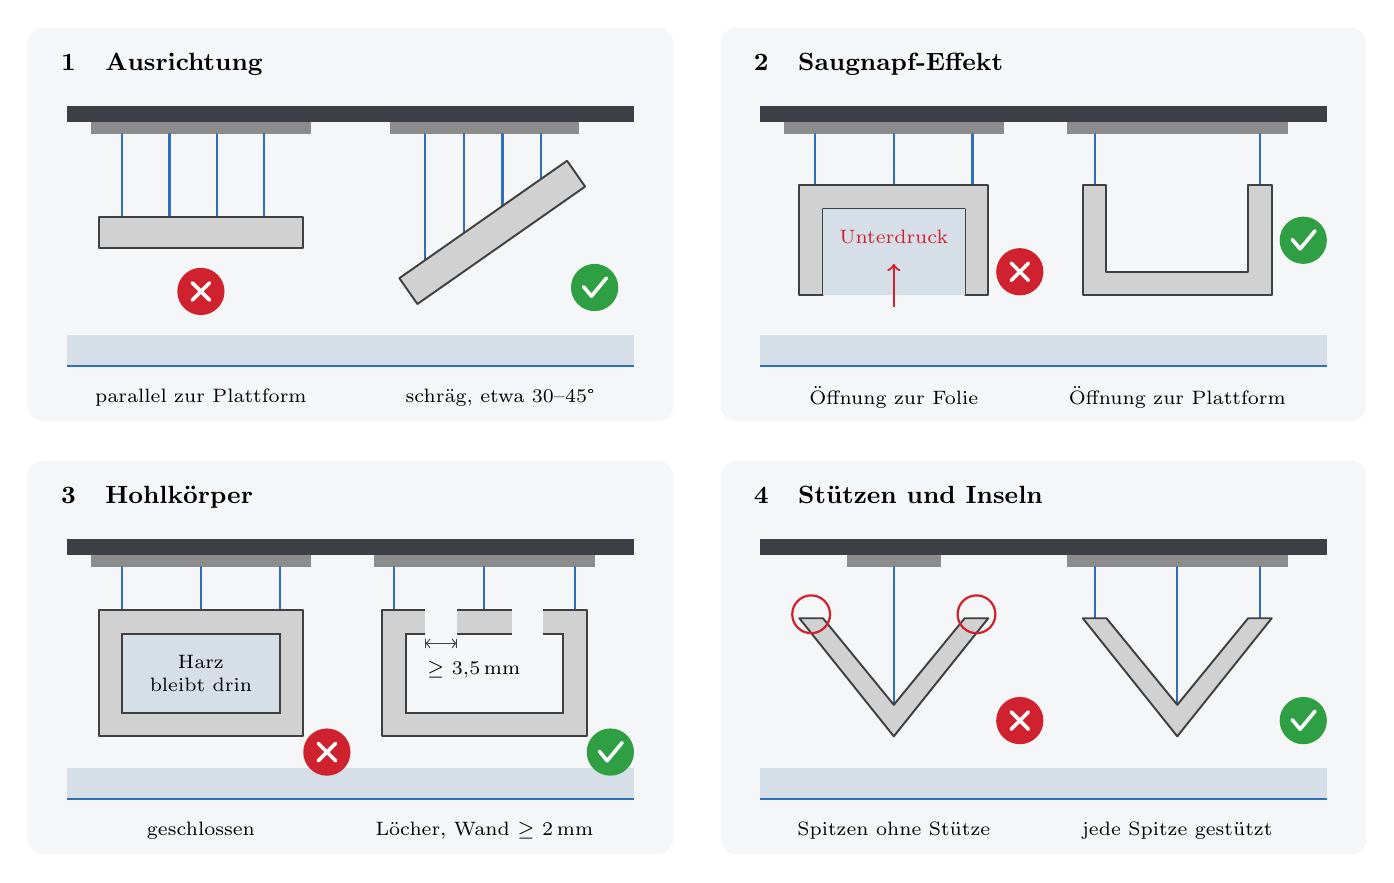
\begin{tikzpicture}[x=1mm, y=1mm, font=\scriptsize,
    teil/.style={fill=black!18, draw=black!75, line width=0.7pt, line join=round},
    stuetzlinie/.style={stuetze, line width=0.8pt, line cap=round},
    ok/.pic={\fill[okgruen] (0,0) circle (3);
      \draw[white, line width=1.3pt, line cap=round, line join=round]
        (-1.4,0.1) -- (-0.4,-1.1) -- (1.5,1.2);},
    nok/.pic={\fill[nokrot] (0,0) circle (3);
      \draw[white, line width=1.3pt, line cap=round]
        (-1.1,-1.1) -- (1.1,1.1) (-1.1,1.1) -- (1.1,-1.1);},
  ]
  \definecolor{okgruen}{RGB}{46,160,67}
  \definecolor{nokrot}{RGB}{207,34,46}
  \definecolor{stuetze}{RGB}{47,111,183}
  \definecolor{feld}{RGB}{244,246,248}
  \definecolor{bett}{RGB}{60,64,70}
  \definecolor{harz}{RGB}{214,222,232}

  % Feldrahmen, Titel, Druckplattform (oben) und Tank mit Folie (unten):
  % \feld{x}{y}{Titel}
  \newcommand{\feld}[3]{%
    \fill[feld, rounded corners=2mm] (#1,#2) rectangle ++(82,50);
    \node[anchor=north west, font=\small\bfseries] at (#1+3,#2+48) {#3};
    \fill[bett] (#1+5,#2+38) rectangle ++(72,2);
    \fill[harz] (#1+5,#2+7) rectangle ++(72,4);
    \draw[stuetze, line width=0.8pt] (#1+5,#2+7) -- ++(72,0);}
  % Raft unter der Druckplattform: \raft{x-links}{x-rechts}
  \newcommand{\raft}[2]{\fill[black!45] (#1,36.5) rectangle (#2,38);}

  % ---------------- 1 Ausrichtung -----------------------------------
  \feld{0}{55}{1\quad Ausrichtung}
  \begin{scope}[shift={(0,55)}]
    % flach: jede Schicht ist die ganze Fläche
    \raft{8}{36}
    \foreach \x in {12,18,24,30} \draw[stuetzlinie] (\x,36.5) -- (\x,26);
    \draw[teil] (9,22) rectangle (35,26);
    \pic at (22,16.5) {nok};
    % schräg: kleine Schichten, geringe Abzugskräfte
    \raft{46}{70}
    \draw[stuetzlinie] (50.5,36.5) -- (50.5,20.5) (55.4,36.5) -- (55.4,23.9)
      (60.3,36.5) -- (60.3,27.4) (65.2,36.5) -- (65.2,30.8);
    \begin{scope}[shift={(59,24)}, rotate=35]
      \draw[teil] (-13,-2) rectangle (13,2);
    \end{scope}
    \pic at (72,17) {ok};
    \node at (22,3) {parallel zur Plattform};
    \node at (60,3) {schräg, etwa 30--45°};
  \end{scope}

  % ---------------- 2 Saugnapf-Effekt -------------------------------
  \feld{88}{55}{2\quad Saugnapf-Effekt}
  \begin{scope}[shift={(88,55)}]
    % Öffnung zur Folie: Unterdruck beim Abziehen
    \raft{8}{36}
    \foreach \x in {12,22,32} \draw[stuetzlinie] (\x,36.5) -- (\x,30);
    \draw[teil] (10,16) -- (10,30) -- (34,30) -- (34,16) -- (31,16) -- (31,27)
      -- (13,27) -- (13,16) -- cycle;
    \fill[harz] (13,16) rectangle (31,27);
    \draw[nokrot, line width=0.8pt, ->] (22,14.5) -- (22,20);
    \node[nokrot] at (22,23.5) {Unterdruck};
    \pic at (38,19) {nok};
    % Öffnung zur Plattform: Harz fließt ab
    \raft{44}{72}
    \foreach \x in {47.5,68.5} \draw[stuetzlinie] (\x,36.5) -- (\x,30);
    \draw[teil] (46,30) -- (46,16) -- (70,16) -- (70,30) -- (67,30) -- (67,19)
      -- (49,19) -- (49,30) -- cycle;
    \pic at (74,23) {ok};
    \node at (22,3) {Öffnung zur Folie};
    \node at (58,3) {Öffnung zur Plattform};
  \end{scope}

  % ---------------- 3 Hohlkörper ------------------------------------
  \feld{0}{0}{3\quad Hohlkörper}
  \begin{scope}
    % geschlossen: Harz bleibt innen eingeschlossen
    \raft{8}{36}
    \foreach \x in {12,22,32} \draw[stuetzlinie] (\x,36.5) -- (\x,31);
    \draw[teil] (9,15) rectangle (35,31);
    \fill[harz, draw=black!75, line width=0.7pt] (12,18) rectangle (32,28);
    \node[align=center] at (22,23) {Harz\\bleibt drin};
    \pic at (38,13) {nok};
    % ausgehöhlt mit Ablauflöchern nahe der Plattform
    \raft{44}{72}
    \foreach \x in {46.5,58,69.5} \draw[stuetzlinie] (\x,36.5) -- (\x,31);
    \draw[teil] (45,15) rectangle (71,31);
    \fill[feld, draw=black!75, line width=0.7pt] (48,18) rectangle (68,28);
    \fill[feld] (50.5,27.6) rectangle (54.5,31.4);
    \fill[feld] (61.5,27.6) rectangle (65.5,31.4);
    \draw[black!75] (50.5,26.2) -- (50.5,27.4) (54.5,26.2) -- (54.5,27.4);
    \draw[<->, black!75] (50.5,26.8) -- (54.5,26.8);
    \node[anchor=north west] at (49.5,25.8) {$\ge$ 3,5\,mm};
    \pic at (74,13) {ok};
    \node at (22,3) {geschlossen};
    \node at (58,3) {Löcher, Wand $\ge$ 2\,mm};
  \end{scope}

  % ---------------- 4 Stützen und Inseln ----------------------------
  \feld{88}{0}{4\quad Stützen und Inseln}
  \begin{scope}[shift={(88,0)}]
    % Spitzen zur Plattform entstehen zuerst und brauchen eine Stütze
    \raft{16}{28}
    \draw[stuetzlinie] (22,36.5) -- (22,19);
    \draw[teil] (10,30) -- (13,30) -- (22,19) -- (31,30) -- (34,30) -- (22,15) -- cycle;
    \draw[nokrot, line width=0.8pt] (11.5,30.5) circle (2.4) (32.5,30.5) circle (2.4);
    \pic at (38,17) {nok};
    \raft{44}{72}
    \draw[stuetzlinie] (58,36.5) -- (58,19) (47.5,36.5) -- (47.5,30)
      (68.5,36.5) -- (68.5,30);
    \draw[teil] (46,30) -- (49,30) -- (58,19) -- (67,30) -- (70,30) -- (58,15) -- cycle;
    \pic at (74,17) {ok};
    \node at (22,3) {Spitzen ohne Stütze};
    \node at (58,3) {jede Spitze gestützt};
  \end{scope}
\end{tikzpicture}

\end{center}

\subsection{Richtwerte für die Konstruktion}

Die folgenden Richtwerte für SLA-Drucke stammen von Protolabs Network. Wähle die Wände bei belasteten Teilen dicker, denn das Harz ist nach dem Nachhärten eher spröde. Ein fehlgeschlagener Druck kann außerdem die Folie beschädigen.

\begin{center}
	\small
	\renewcommand{\arraystretch}{1.25}
	\begin{tabularx}{\textwidth}{|l|l|X|}
		\hline
		\textbf{Merkmal} & \textbf{Richtwert} & \textbf{Hinweis} \\ \hline
		Wand, an mindestens zwei Seiten verbunden & $\ge$ 0,4\,mm & \\ \hline
		Freistehende Wand & $\ge$ 0,6\,mm & Übergang zur Basis abrunden. \\ \hline
		Überhang ohne Stütze & $\le$ 1\,mm & mindestens 19$^\circ$ zur Waagerechten \\ \hline
		Brücke ohne Stütze & $\le$ 21\,mm & \\ \hline
		Erhabene Details (Schrift) & $\ge$ 0,1\,mm hoch & \\ \hline
		Vertiefte Details (Gravur) & $\ge$ 0,4\,mm breit und tief & Sonst laufen sie zu. \\ \hline
		Loch & $\ge$ 0,8\,mm & Kleinere Löcher wachsen zu. \\ \hline
		Senkrechter Stift, Draht & $\ge$ 1,5\,mm & dünner nur mit Stütze \\ \hline
		Spiel bewegliche Teile & 0,5\,mm & \\ \hline
		Spiel gefügte Teile & 0,2\,mm & Presspassung: 0,1\,mm \\ \hline
		Abstand zwischen Teilen & $\ge$ 1\,mm & \\ \hline
		Ablaufloch bei Hohlkörpern & $\ge$ 3,5\,mm & mindestens eins pro Hohlraum \\ \hline
		Wand beim Aushöhlen & $\ge$ 2\,mm & \\ \hline
	\end{tabularx}
\end{center}

\section{Modell in Lychee Slicer vorbereiten}

Damit ein Modell gedruckt werden kann, muss es in Schichten umgerechnet werden (Slicen). Dafür verwenden wir \textit{Lychee Slicer}. Die Arbeitsschritte findest du oben in der Mitte: \textit{Layout} (Modell platzieren), \textit{Prepare} (Stützen, Raft, Aushöhlen) und \textit{Exportieren}.

\IfFileExists{zeichnungen/LycheeSlicer.png}{%
\begin{figure}[H]
	\centering
	% Markierungen: Koordinaten relativ zum Bild (0,0 = unten links, 1,1 = oben rechts)
	\begin{tikzpicture}[marke/.style={circle, draw=black, fill=white, line width=1pt, minimum size=4.8mm, inner sep=0pt, font=\bfseries\small}]
		\node[anchor=south west, inner sep=0pt] (bild) at (0,0) {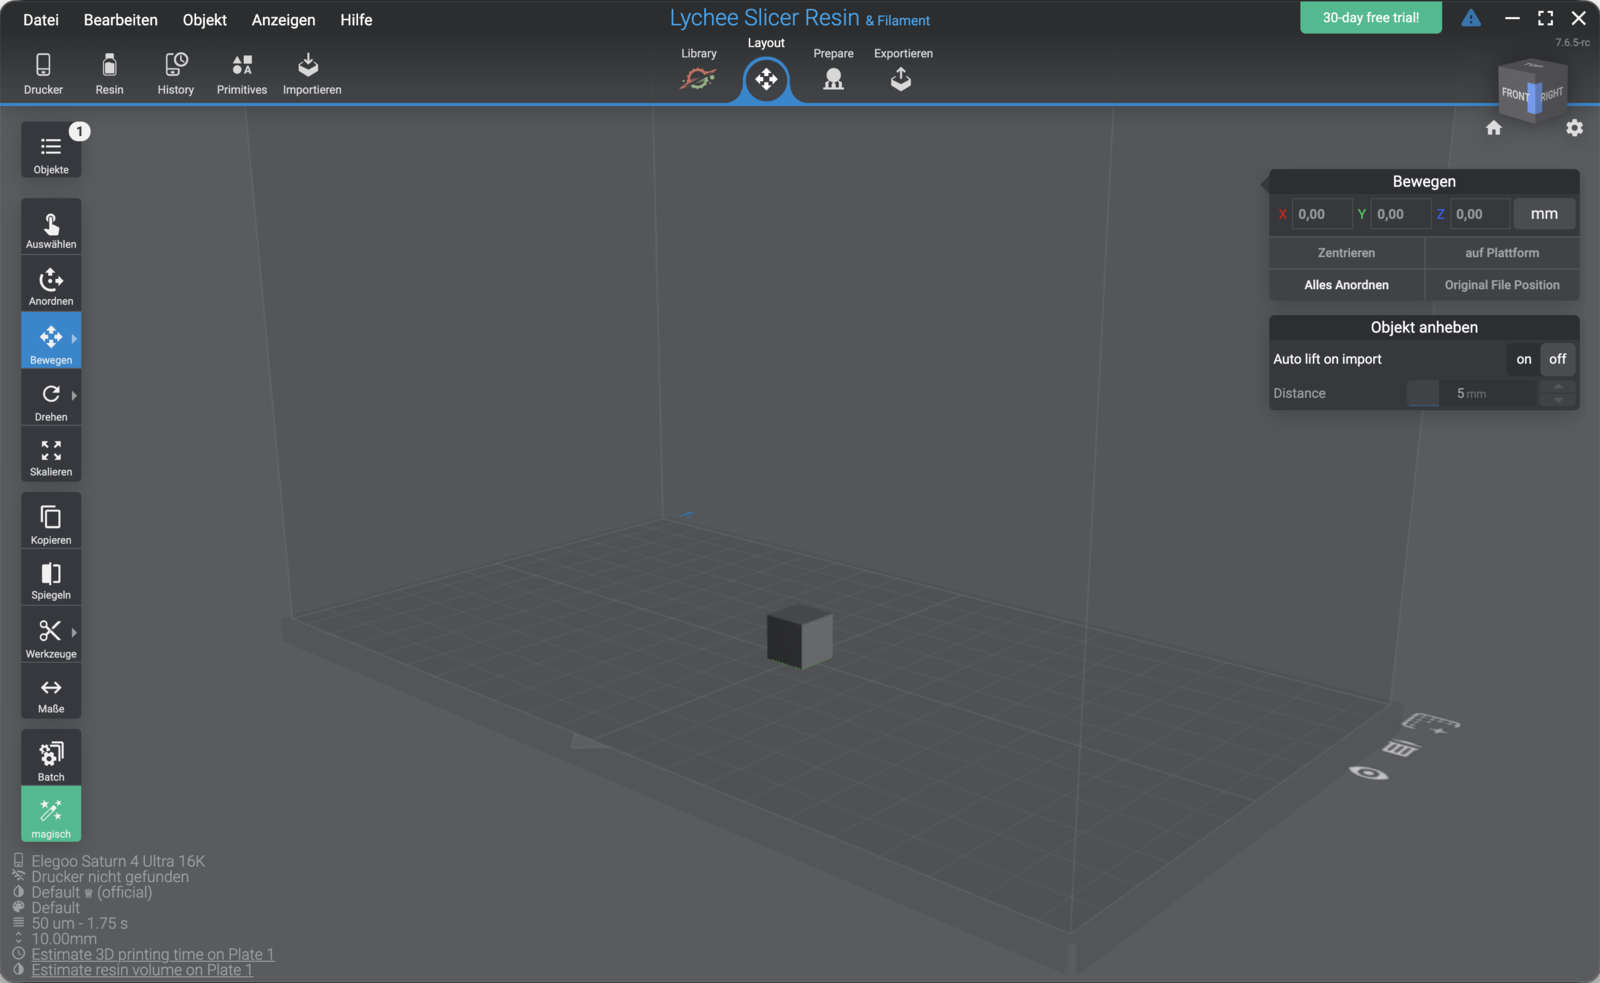
\includegraphics[width=\textwidth]{zeichnungen/LycheeSlicer.png}};
		\begin{scope}[x={(bild.south east)}, y={(bild.north west)}]
			\begin{scope}[line width=1pt, white]
				\draw (0.092, 0.843) -- (0.027, 0.901);
				\draw (0.130, 0.843) -- (0.069, 0.901);
				\draw (0.479, 0.843) -- (0.479, 0.900);
				\draw (0.521, 0.843) -- (0.521, 0.908);
				\draw (0.563, 0.843) -- (0.563, 0.908);
				\draw (0.084, 0.598) -- (0.051, 0.598);
			\end{scope}
			\node[marke] at (0.092, 0.843) {1};
			\node[marke] at (0.130, 0.843) {2};
			\node[marke] at (0.479, 0.843) {3};
			\node[marke] at (0.521, 0.843) {4};
			\node[marke] at (0.563, 0.843) {5};
			\node[marke] at (0.084, 0.598) {6};
			\node[marke] at (0.200, 0.079) {7};
		\end{scope}
	\end{tikzpicture}
	\caption{Lychee Slicer: Drucker \textcircled{\small 1}, Harzprofil \textcircled{\small 2}, Arbeitsschritte \textit{Layout} \textcircled{\small 3}, \textit{Prepare} \textcircled{\small 4} und \textit{Exportieren} \textcircled{\small 5}, Bewegen/Drehen/Skalieren \textcircled{\small 6}, Statusanzeige mit Drucker, Harzprofil, Schichtdicke und Harzverbrauch \textcircled{\small 7}. Im Bild ist noch ein anderer Drucker eingestellt, bei uns muss dort \textit{UniFormation GKtwo} stehen.}
	\label{abb.lychee}
\end{figure}}{}

\subsection{Drucker und Harz einstellen}

\begin{itemize}
	\item Wähle oben links unter \textit{Drucker} \textcircled{\small 1} den \textbf{UniFormation GKtwo} und unter \textit{Resin} \textcircled{\small 2} das im FabLab angelegte Harzprofil \textbf{Phrozen Water-Washable Rapid Black}.
	\item Kontrolliere in der Statusanzeige unten links \textcircled{\small 7} den Drucker, das Harzprofil und die Schichtdicke von 50\,µm. Belichtungszeiten und Schichtdicke sind im Profil fest eingestellt und werden nur nach Absprache mit dem Maschinenverantwortlichen geändert.
	\item Lade dein Modell per Drag-and-Drop, über \textit{Importieren} oder über \textit{Datei} \ra{} \textit{Öffnen}.
	\item Ist das Modell in Zoll angelegt, prüfe nach dem Laden die Größe und rechne es mit \textit{Skalieren} auf Millimeter um (Faktor 25,4).
\end{itemize}

\subsection{Layout: Ausrichten}

Im Schritt \textit{Layout} \textcircled{\small 3} platzierst du das Modell mit den Werkzeugen am linken Rand.

\begin{itemize}
	\item \textbf{Ausrichten:} Stelle das Teil mit \textit{Bewegen}, \textit{Drehen} und \textit{Skalieren} \textcircled{\small 6} in der Regel \textbf{schräg} (etwa 30--45$^\circ$). So wird jede Schicht kleiner, die Abzugskräfte sinken, und es entstehen keine Saugnäpfe. Lege große ebene Flächen nicht parallel zur Druckplattform. Drehe Sichtflächen möglichst von der Plattform weg, denn die Stützen hinterlassen Spuren.
	\item Mehrere Teile verteilst du mit \textit{Anordnen} bzw.\ \textit{Alles Anordnen}. Halte dabei mindestens 1\,mm Abstand.
\end{itemize}

\subsection{Prepare: Stützen, Raft und Aushöhlen}

Im Schritt \textit{Prepare} \textcircled{\small 4} (Abbildung~\ref{abb.lychee}) legst du Stützen, Raft und Hohlräume an. Die Bereiche wählst du am linken Rand aus, die zugehörigen Einstellungen erscheinen rechts. Die Nummern im folgenden Text beziehen sich auf Abbildung~\ref{abb.lychee-prepare}.

\begin{figure}[H]
	\centering
	\begin{tikzpicture}[marke/.style={circle, draw=black, fill=white, line width=1pt, minimum size=4.8mm, inner sep=0pt, font=\bfseries\small}]
		\node[anchor=south west, inner sep=0pt] (bild) at (0,0) {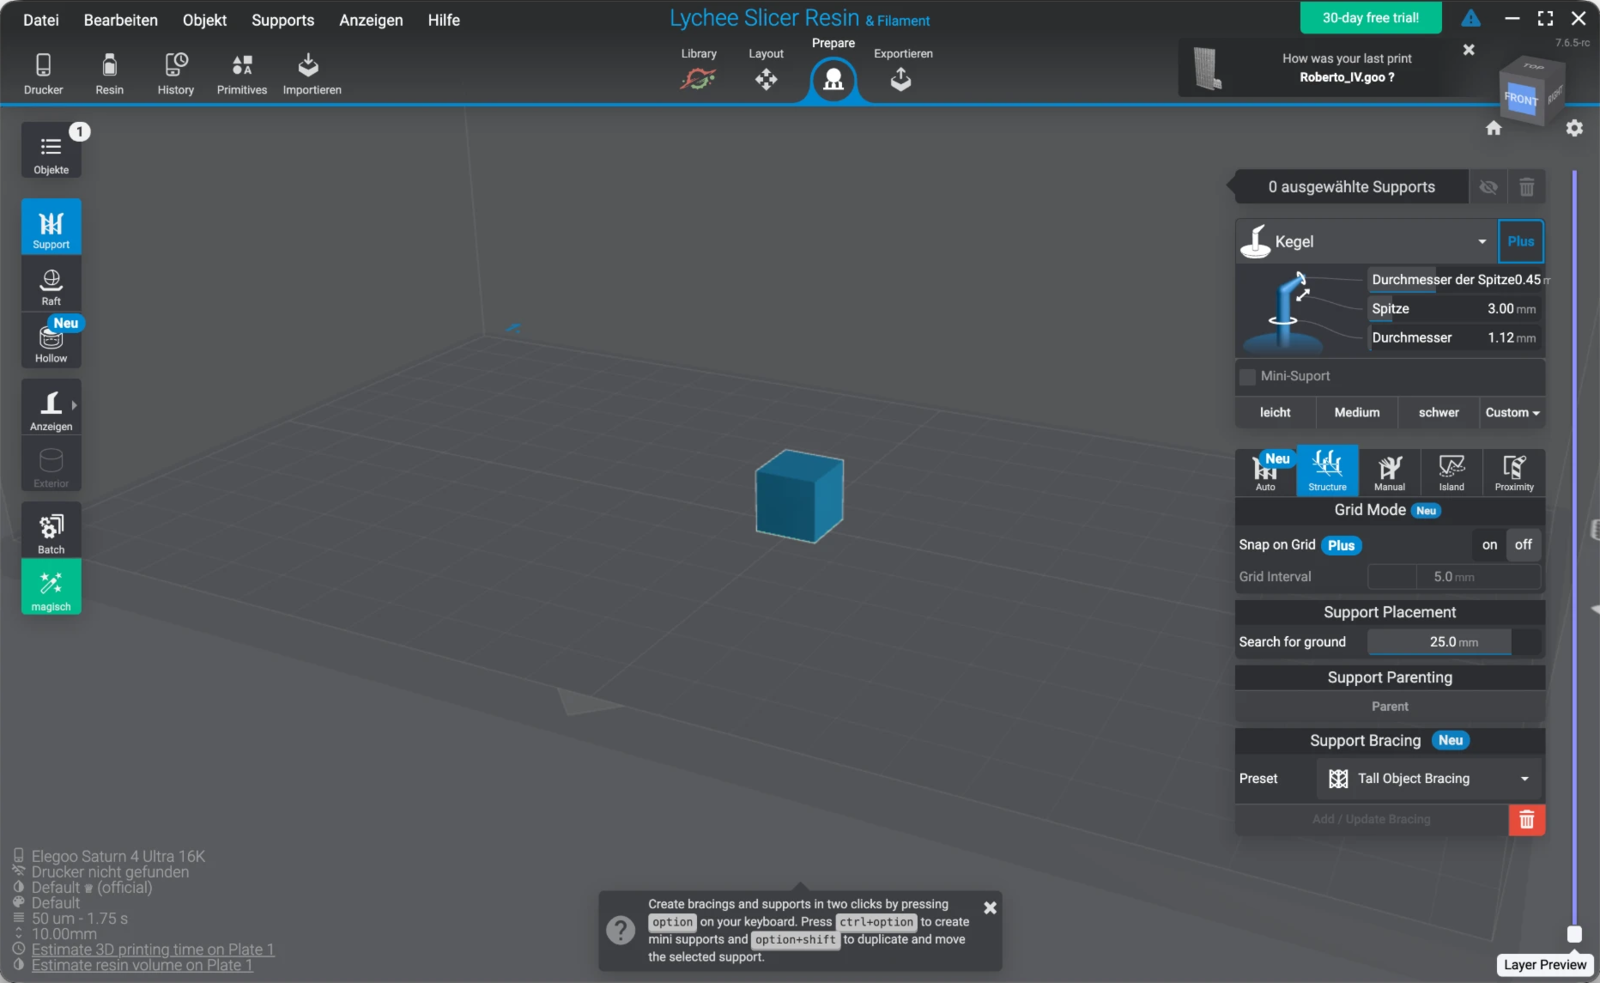
\includegraphics[width=\textwidth]{zeichnungen/LycheePrepare.png}};
		\begin{scope}[x={(bild.south east)}, y={(bild.north west)}]
			\begin{scope}[line width=1pt, white]
				\draw (0.079, 0.770) -- (0.051, 0.770);
				\draw (0.079, 0.709) -- (0.051, 0.709);
				\draw (0.079, 0.651) -- (0.051, 0.651);
				\draw (0.747, 0.520) -- (0.773, 0.520);
				\draw (0.747, 0.581) -- (0.773, 0.581);
				\draw (0.932, 0.473) -- (0.907, 0.502);
			\end{scope}
			\node[marke] at (0.079, 0.770) {1};
			\node[marke] at (0.079, 0.709) {2};
			\node[marke] at (0.079, 0.651) {3};
			\node[marke] at (0.747, 0.520) {4};
			\node[marke] at (0.747, 0.581) {5};
			\node[marke] at (0.932, 0.473) {6};
		\end{scope}
	\end{tikzpicture}
	\caption{Lychee Slicer, Schritt \textit{Prepare}: Stützen \textcircled{\small 1}, Raft \textcircled{\small 2}, Aushöhlen \textcircled{\small 3}, automatische Stützen \textcircled{\small 4}, Stützenstärke \textcircled{\small 5}, Inselerkennung \textcircled{\small 6}}
	\label{abb.lychee-prepare}
\end{figure}

\begin{itemize}
	\item \textbf{Aushöhlen:} Massive Teile höhlst du unter \textit{Hollow} \textcircled{\small 3} aus und setzt Ablauflöcher (siehe Abschnitt~\ref{sec:druckbarkeit}). Das spart Harz und damit Geld. Höhle das Teil zuerst aus und erzeuge erst danach die Stützen.
	\item \textbf{Stützen:} Unter \textit{Support} \textcircled{\small 1} erzeugst du mit \textit{Auto} \textcircled{\small 4} die Stützen automatisch. Die Stärke \textcircled{\small 5} bleibt in der Regel auf \textit{Medium}, für große, schwere Teile wählst du \textit{schwer}.
	\item \textbf{Inseln prüfen:} Die Inselerkennung \textit{Island} \textcircled{\small 6} zeigt Stellen, die ohne Stütze in der Luft entstehen würden. Ergänze dort von Hand Stützen.
	\item \textbf{Raft:} Wähle unter \textit{Raft} \textcircled{\small 2} den Raft \textbf{unten rechts} (siehe Abbildung~\ref{abb.lychee-raft}). Die mit \textit{Plus} markierten Rafts gibt es in der kostenlosen Version von Lychee, die wir verwenden, nicht. Der Raft haftet an der Druckplattform und trägt die Stützen. Drucke deshalb nie direkt auf die Plattform.
\end{itemize}

\begin{figure}[H]
	\centering
	\begin{tikzpicture}
		\node[anchor=south west, inner sep=0pt] (bild) at (0,0) {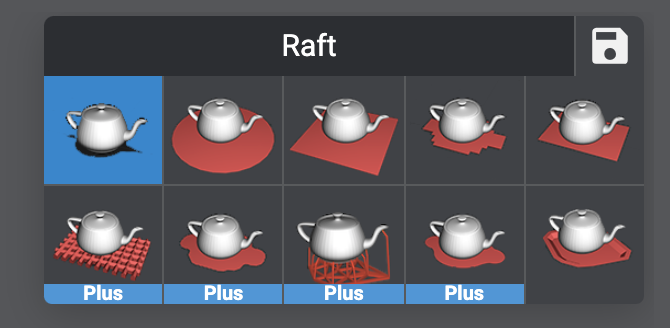
\includegraphics[width=0.5\textwidth]{zeichnungen/LycheeRaft.png}};
		\begin{scope}[x={(bild.south east)}, y={(bild.north west)}]
			\draw[line width=2pt, yellow] (0.784, 0.076) rectangle (0.960, 0.430);
		\end{scope}
	\end{tikzpicture}
	\caption{Raft-Auswahl in Lychee: Raft unten rechts verwenden}
	\label{abb.lychee-raft}
\end{figure}

\subsection{Exportieren auf den USB-Stick}

\begin{itemize}
	\item Erzeuge im Schritt \textit{Exportieren} \textcircled{\small 5} (Abbildung~\ref{abb.lychee}) die Druckdatei und speichere sie auf dem \textbf{USB-Stick des Druckers}. Wähle einen eindeutigen Dateinamen, z.\,B. \enquote{Max\_Mustermann\_Dateiname}.
	\item Lass dir unten links \textcircled{\small 7} (Abbildung~\ref{abb.lychee}) mit \textit{Estimate resin volume} den \textbf{Harzverbrauch in ml} anzeigen und \textbf{notiere ihn}. Du brauchst ihn zum Bezahlen. Daneben kannst du auch die Druckzeit abschätzen lassen.
	\item Der Drucker ist \textbf{nicht im Netzwerk}. Druckdateien kommen nur per USB-Stick auf den Drucker.
\end{itemize}

\newpage

\section{Drucken}

\subsection{Vorbereitung am Drucker}

\begin{itemize}
	\item Zieh die Schutzbrille und die Nitrilhandschuhe an.
	\item Nimm die grüne Haube ab und prüfe:
	\begin{itemize}
		\item Ist die Druckplattform sauber und mit dem Schnellspanner fest eingesetzt?
		\item Liegen keine ausgehärteten Reste oder Teile eines Fehldrucks im Tank? Frag im Zweifel einen Betreuer.
		\item Ist genug Harz im Tank? Der Füllstand muss für den angezeigten Verbrauch reichen und darf die MAX-Markierung nicht überschreiten.
	\end{itemize}
	\item Rühre das Harz im Tank vorsichtig mit dem Silikonspatel um, damit sich abgesetzte Farbpigmente verteilen. Kratze dabei nicht an der Folie.
	\item Setze die Haube wieder auf.
\end{itemize}

\subsection{Druck starten}

\begin{itemize}
	\item Steck den USB-Stick in den Drucker.
	\item Wähle am Touchscreen deine Druckdatei aus. Sie wird zuerst in den internen Speicher des Druckers kopiert.
	\item Prüfe die Vorschau, die Druckzeit und den Harzverbrauch und starte den Druck.
	\item Der GKtwo heizt den Tank vor und beginnt erst, wenn das Harz die eingestellte Temperatur erreicht hat.
	\item Leg den USB-Stick zurück an seinen Platz.
	\item Wenn du nicht bis zum Druckende bleibst, klebe einen Post-it mit deinem Namen und deiner E-Mail-Adresse an den Drucker. Der Druck darf über Nacht laufen.
\end{itemize}

\subsection{Druck abbrechen}

\begin{itemize}
	\item Brich den Druck am Display des Druckers ab (\textit{Stopp}), wenn sichtbar Teile abgerissen sind, ungewöhnliche Geräusche auftreten, eine Fehlermeldung erscheint oder Harz ausläuft.
	\item Warte nach dem Abbruch, bis die Plattform stillsteht, und \textbf{informiere einen Betreuer}. Abgerissene Teile im Tank können beim nächsten Druck die Folie und das LCD beschädigen.
\end{itemize}

\section{Nachbearbeitung}

Trage ab jetzt immer die \textbf{Schutzbrille} und die \textbf{Nitrilhandschuhe}. Gewaschen wird im \textbf{Form Wash}, nachgehärtet im \textbf{Form Cure}. Da das Harz wasserwaschbar ist, ist der Form Wash \textbf{mit Wasser statt mit Isopropanol} gefüllt.

\begin{enumerate}
	\item \textbf{Abtropfen lassen:} Nach dem Druckende fährt die Plattform nach oben. Warte einige Minuten, bis das Harz in den Tank zurückgetropft ist.
	\item \textbf{Plattform abnehmen:} Nimm die Haube ab, löse den Schnellspanner und nimm die Plattform leicht schräg über dem Tank heraus. Setze die Haube sofort wieder auf, damit kein Licht an das Harz kommt.
	\item \textbf{Teile ablösen:} Leg die Plattform auf die Unterlage. Schieb den Spachtel flach unter den Raft und löse die Teile ab. Führe den Spachtel dabei \textbf{immer vom Körper weg}.
	\item \textbf{Waschen im Form Wash:} Leg die Teile in den Korb. Stelle am Form Wash mit dem Dreh-Drück-Knopf die Zeit auf \textbf{1 Minute} und wähle \textit{Start}. Der Korb fährt ins Wasser und nach Ablauf der Zeit wieder heraus. Wasche nicht länger, sonst leidet die Oberfläche. Fahre den Korb danach mit \textit{Sleep} wieder ein.
	\item \textbf{Trocknen:} Lass die Teile mindestens \textbf{30 Minuten} trocknen oder trockne sie mit Druckluft. Entferne das Wasser auch aus Hohlräumen und Ablauflöchern. Nasse Teile dürfen nicht nachgehärtet werden, sonst entstehen weiße Flecken und Risse.
	\item \textbf{Stützen entfernen:} Entferne die Stützen am besten vor dem Nachhärten. Dann sind sie noch weich und brechen sauber ab. Nimm dafür einen Seitenschneider oder eine Zange.
	\item \textbf{Nachhärten im Form Cure:} Leg die Teile auf den Drehteller, stelle am Form Cure die Zeit auf \textbf{15 Minuten} \textbf{ohne Heizen} (Temperatur aus) und starte. Härte nicht deutlich länger, sonst werden die Teile spröde.
	\item \textbf{Plattform reinigen:} Wisch die Harzreste mit einem Papiertuch von der Druckplattform, reinige die Plattform mit Wasser, trockne sie ab und setze sie wieder in den Drucker ein.
\end{enumerate}

Lass harzverschmierte Papiertücher und Handschuhe erst in der Sonne oder unter UV-Licht aushärten und wirf sie dann in den Restmüll.

\section{Bezahlen und Abschließen}

\begin{itemize}
	\item Räum deinen Arbeitsplatz auf: Säubere den Spachtel, die Behälter und die Unterlage und nimm Harzflecken sofort mit einem Papiertuch auf.
	\item Bezahlt wird der in Lychee angezeigte Harzverbrauch in \textbf{ml}. Runde ihn am Kassenterminal auf ganze ml auf.
	\item \textbf{Fehldrucke müssen ebenfalls bezahlt werden.}
	\item Melde Probleme oder Schäden einem Betreuer.
\end{itemize}

\section{Infos für Betreuer}

\subsection{Harz}

\begin{itemize}
	\item Die Harzflasche vor dem Nachfüllen gut schütteln und erst dann in den Tank füllen. Der Füllstand reicht höchstens bis zur MAX-Markierung.
	\item Nach einem Fehldruck oder vor einer längeren Pause das Harz durch einen Papierfilter zurück in die Flasche gießen und den Tank reinigen.
	\item Das Harz unter Verschluss, dunkel und bei 15--35\,\textcelsius{} lagern.
\end{itemize}

\subsection{Waschwasser im Form Wash}

\begin{itemize}
	\item Der Form Wash ist mit \textbf{Wasser} gefüllt, nicht mit Isopropanol. Die Tauchspindel des Form Wash ist auf Isopropanol ausgelegt und hier nicht aussagekräftig.
	\item Das Waschwasser wechseln, wenn es deutlich trüb ist oder die Teile klebrig bleiben.
	\item Altes Waschwasser \textbf{nicht in den Abfluss} gießen, sondern in einem offenen, durchsichtigen Behälter einige Tage in die Sonne oder unter UV-Licht stellen, bis das gelöste Harz ausgehärtet ist und sich abgesetzt hat. Die festen Reste abfiltern und im Restmüll entsorgen.
\end{itemize}

\subsection{nFEP-Folie}

\begin{itemize}
	\item Die Folie vor jedem Druck auf Kratzer, Dellen, Löcher und Trübung prüfen. Bei Beschädigung tauschen, sonst kann Harz auf das LCD laufen.
	\item Fingerabdrücke und Schlieren auf der Unterseite der Folie mit etwas Isopropanol und einem fusselfreien Tuch abwischen.
	\item Ausgehärtete Reste im Tank vorsichtig mit dem Silikonspatel lösen, niemals mit Werkzeug aus Metall.
\end{itemize}

\subsection{Typische Fehler}

\begin{itemize}
	\item \textbf{Nichts haftet an der Plattform:} die Plattform nivellieren, Harztemperatur und Belichtung der ersten Schichten prüfen und den Tank auf Reste kontrollieren.
	\item \textbf{Teile abgerissen, Stücke im Tank:} das Harz filtern, den Tank reinigen und Stützen und Ausrichtung im Slicer verbessern.
	\item \textbf{Löcher oder Risse in Hohlkörpern:} Ursache ist meist der Saugnapf-Effekt oder fehlende Ablauflöcher.
	\item \textbf{Weiße Flecken nach dem Nachhärten:} Die Teile waren beim Härten noch nass.
\end{itemize}

\subsection{Wartungsintervalle}

Folie, LCD-Schutzfolie und Filter werden nur bei ausgeschaltetem Drucker getauscht. Zum Nivellieren muss der Drucker dagegen eingeschaltet sein; dabei gilt die Anleitung von UniFormation.

\begin{center}
	\small
	\renewcommand{\arraystretch}{1.3}
	\begin{tabularx}{\textwidth}{|l|l|X|}
		\hline
		\textbf{Bauteil} & \textbf{Intervall} & \textbf{Maßnahme} \\ \hline
		nFEP-Folie & vor jedem Druck & Sichtprüfung, bei Beschädigung oder starker Trübung tauschen. \\ \hline
		Harz im Tank & vor jedem Druck & Umrühren. Nach Fehldrucken filtern. \\ \hline
		Druckplattform & nach jedem Druck & Reinigen. Bei Haftungsproblemen neu nivellieren. \\ \hline
		Waschwasser & bei Trübung & Wechseln und alten Inhalt aushärten, siehe oben. \\ \hline
		LCD-Schutzfolie & bei Bedarf & Bei Kratzern oder Harz auf dem LCD tauschen. \\ \hline
		Aktivkohlefilter & alle 3 Monate & Filter hinten am Drucker tauschen. \\ \hline
		Z-Achse & alle 3 Monate & Gewindespindel und Führung reinigen und dünn fetten. \\ \hline
	\end{tabularx}
\end{center}

\noindent\begin{minipage}{0.75\textwidth}
	Anleitungen und Videos von UniFormation zum Nivellieren, Folienwechsel, Tausch der LCD-Schutzfolie und Filtern des Harzes: \href{https://uniformation3d.com/pages/gktwo-guide}{GKtwo Guide}
\end{minipage}\hfill
\qrcode[height=2cm]{https://uniformation3d.com/pages/gktwo-guide}

\ccLicense{sla-drucker-einweisung}{Einweisung SLA-Drucker}

\end{document}
